\chapter{Diboson resonances as signature for new physics}
\label{ch:dibosonIntro}

This part of the thesis is dedicated to the description and discussion of searches for new physics in proton-proton collision data collected with the CMS experiment at LHC.
As pointed out in Chapter~\ref{ch:theory}, the remarkable compatibility of the discovered scalar resonance by the ATLAS and CMS collaborations with the SM predictions for the Higgs boson,
force physicists to deeply understand the role of naturalness in the dynamics of this particle.
Several theoretical extensions to the SM have been proposed offering a concrete realization of naturalness,
where new particles with masses in the TeV range generate loop corrections with the necessary cancellations to stabilize the Higgs boson mass.
%This means that particular attention can be payed to direct experimental manifestations of new physics represented by the production of these heavy particles.
More natural solutions can therefore be probed at the LHC through the direct discovery of these new, heavy particles in final states with SM objects with known properties.
The research described in this work follows exactly this approach and it is focused on the direct search for new massive resonances decaying to
pairs of vector bosons (WW, WZ, or ZZ) or to a vector boson and a Higgs boson (WH or ZH).
These decay modes can have large branching fractions in several BSM models. 
Popular examples include the bulk scenario of the Randall--Sundrum warped extra-dimentions model described in Section~\ref{subsec:graviton},
as well as the composite Higgs and littlest Higgs models discussed in Section~\ref{subsec:composite}.
Furthermore, the heavy vector triplet model (Section~\ref{subsec:hvt}) generalizes a large class of explicit theories that predict new heavy spin-1 vector bosons,
adopting a simplified model strategy. The two HVT models A and B are considered, which correspond, respectively, to a weakly- and a strongly-coupled theoretical option.
In this context, spin-1 resonances are studied that couple both as a vector triplet ($\PVpr = \Wpr$ and \Zpr) and as singlets (\Wpr or \Zpr), i.e. only a charged or a neutral resonance is expected at a given mass.
The properties of the above benchmark models studied in this thesis are summarized in Table~\ref{tab:models}.\\

\begin{table}[!htb]
\centering
\caption{Summary of the properties of the heavy-resonance models considered in the combination. The polarization of the produced W and Z bosons in these models is mostly longitudinal, as decays to transverse polarizations are suppressed.}
\resizebox{\textwidth}{!}{
\begin{tabular}{cccccc}
\hline
Model & Particles & Spin & Charge & Main production & Main decay \\
\hline
\multirow{3}{*}{HVT model A, $g_\mathrm{V} = 1$} & \Wpr singlet & 1 & $\pm1$ & $\qqbar^\prime$ & $\qqbar^\prime$ \\ 
                                                                                 & \Zpr singlet & 1 & 0 & $\qqbar$ &  $\qqbar$\\
                                                                                 & \Wpr and \Zpr triplet & 1 & $\pm1$,0 & $\qqbar^\prime$,$\qqbar$ & $\qqbar^\prime$,$\qqbar$\\
\hline
\multirow{3}{*}{HVT model B, $g_\mathrm{V} = 3$} & \Wpr singlet & 1 & $\pm1$ & $\qqbar^\prime$ & WZ,WH \\ 
                                                                                 & \Zpr singlet & 1 & 0& $\qqbar$ &  WW,ZH \\
                                                                                 & \Wpr and \Zpr triplet & 1 & $\pm1$,0 & $\qqbar^\prime$,$\qqbar$ & WZ,WH,WW,ZH\\
\hline
%2 / neutral / $G_{\text{RS1}}$ & subdominantly WW, ZZ & mainly $\qqbar$ and $gg$ \\
RS bulk, $\tilde{k}=0.5$ & $\rm G_{bulk}$ & 2 & 0 & $gg$ & WW, ZZ \\
\hline
\end{tabular}}
\label{tab:models}
\end{table}

The signal under investigation is a narrow resonance, referring to the assumption
that the resonance's natural width is smaller than the experimental resolution, covering a large fraction of the parameter space of the reference models considered.
%that the resonance's natural width has a negligible impact on the distribution of the resonance mass reconstructed in the detector.
This assumption allows a ``model-independent'' type of search, where the description of the resonance mass distribution can be restricted to the detector effects only and hence,
independently from the chosen benchmark model.

The semi-leptonic final states are considered, where one of the two bosons is a W decaying into a charged lepton ($\ell$) and a neutrino ($\Pgn$).
The lepton can be either a muon ($\mu$) or an electron (e), although the results include the $\PW\to\tau\Pgn$ contribution from the decay $\tau\to\ell\Pgn\bar{\Pgn}$.
However, the gain in sensitivity from $\tau$ leptons is limited by the small branching fractions involved.
The second boson in the final state decays into quarks, and can be either a vector boson V = W or Z,
or a Higgs boson. In the first case, the final state is labelled as $\ell\Pgn\qqbar$ including $\PW\to\qqbar^\prime$ and $\PZ\to\qqbar$ decays (Figures~\ref{fig:FDsignals_a},~\ref{fig:FDsignals_b} and~\ref{fig:FDsignals_c}).
For the Higgs boson, the final state is labeled as $\ell\Pgn\bbbar$ referring to the Higgs boson decay into a bottom quark-antiquark pair (Fig.~\ref{fig:FDsignals_d}).
Each quark from the V or H boson decays results in a shower of hadrons in the final state called a \textit{jet}. These particles are collected through a jet algorithm which allows to reconstruct the kinematics of the original quark.
These final states provide high sensitivity to this search as the presence of the lepton in the final state highly suppresses the QCD background, while the large branching fractions of the dominant $\PV\to\qqbarpr$ and $\PH\to\bbbar$ decay modes allow to maintain high signal cross sections.

\begin{figure}[!htb]
\centering
\subfigure[]{\label{fig:FDsignals_a}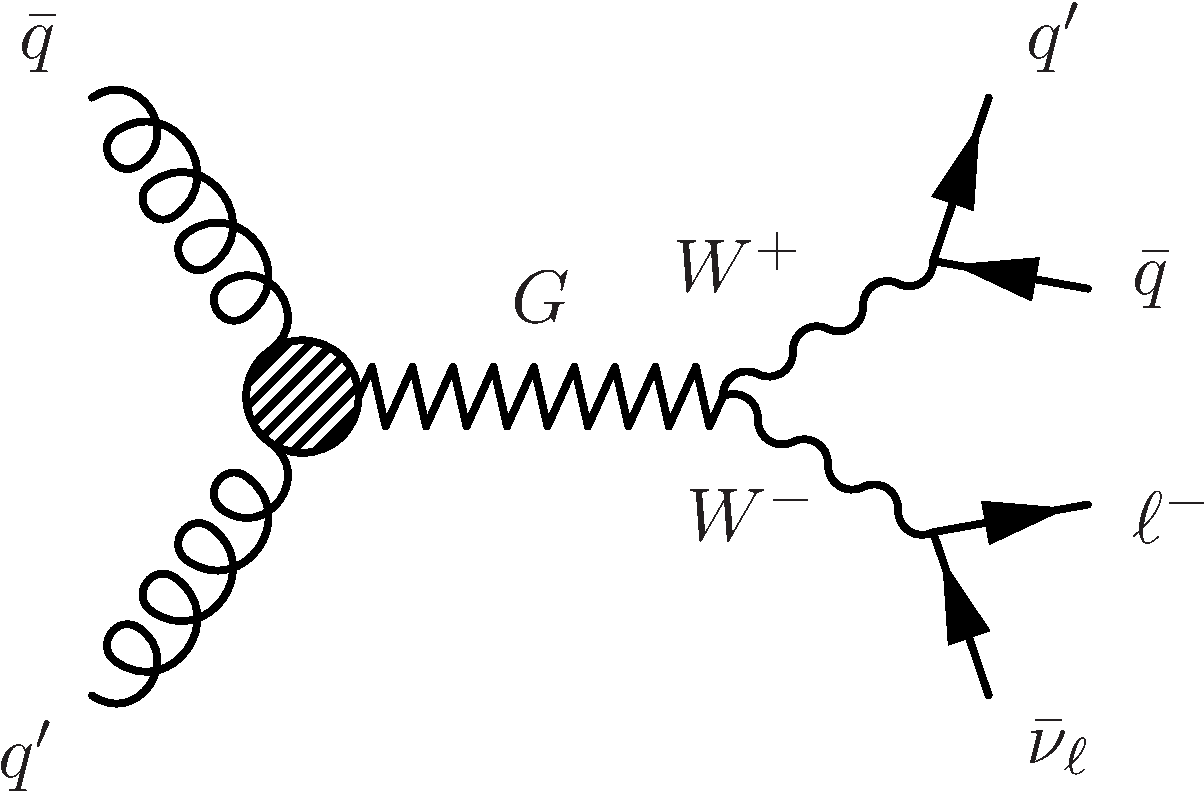
\includegraphics[width=0.3\textwidth]{\chfour/BulkGWW_LO.pdf}}\hspace{1cm}
\subfigure[]{\label{fig:FDsignals_b}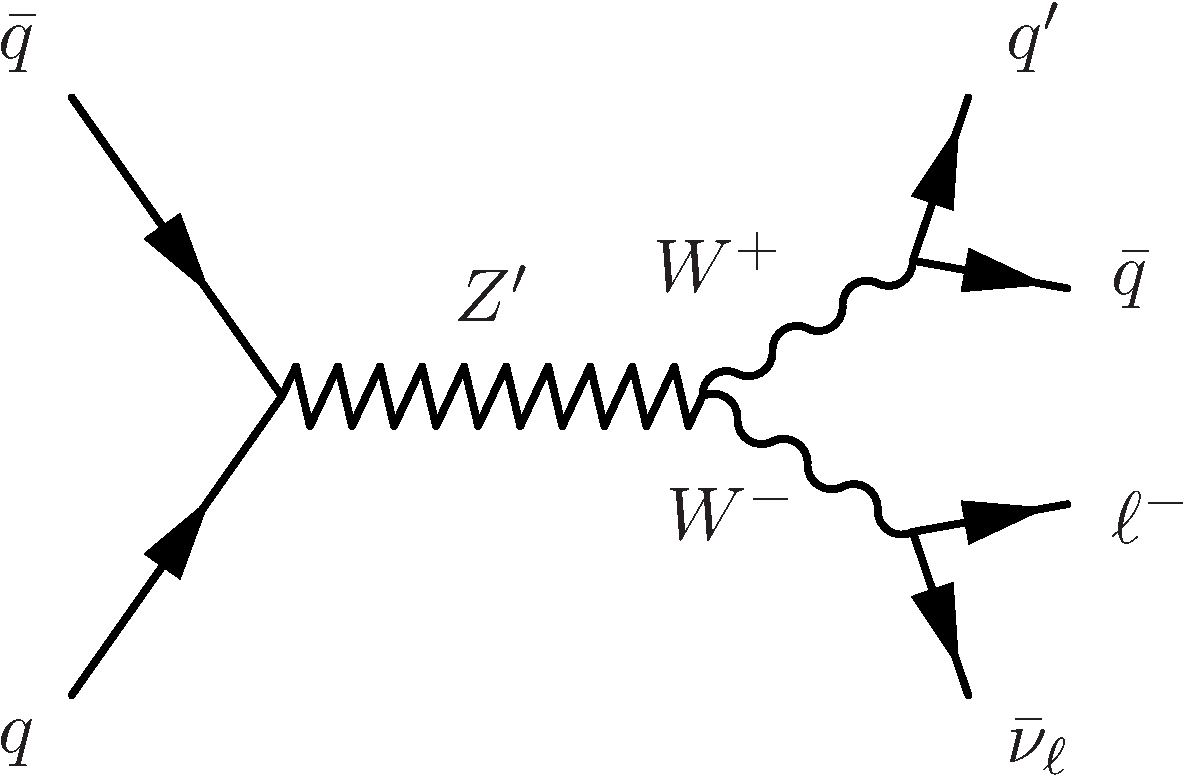
\includegraphics[width=0.3\textwidth]{\chfour/ZprimeWW_LO.pdf}}\\
\subfigure[]{\label{fig:FDsignals_c}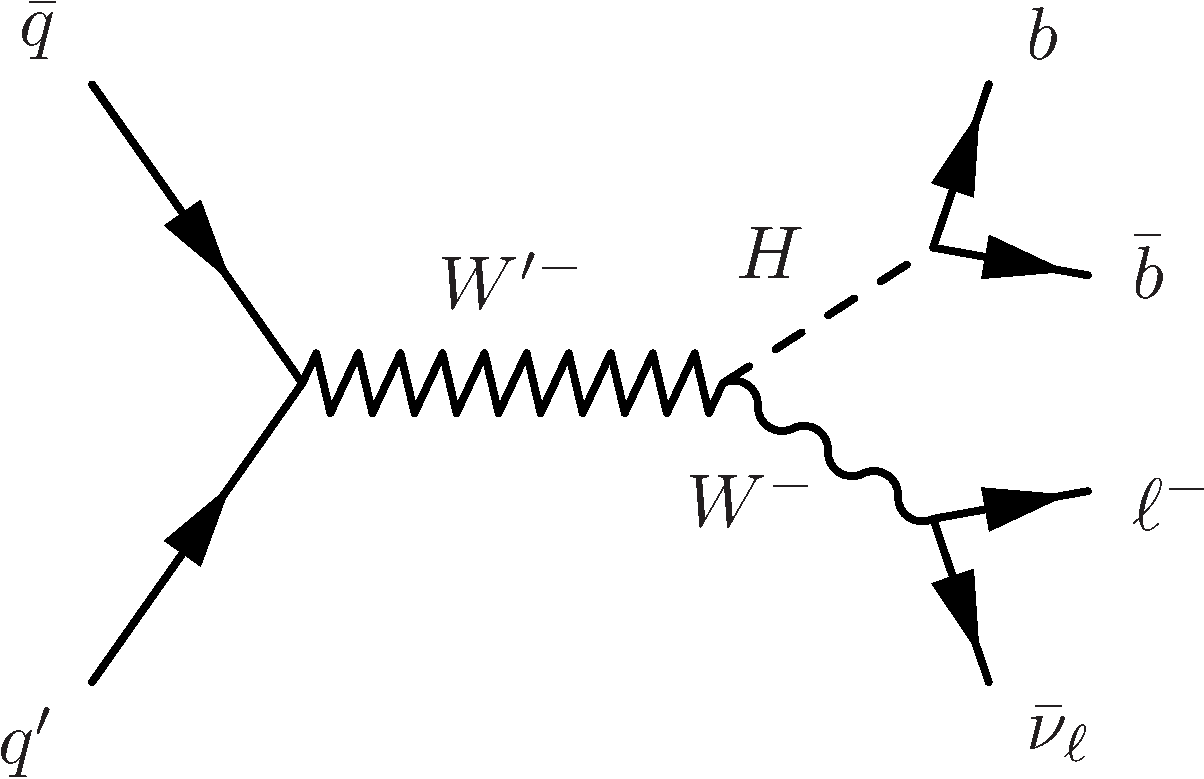
\includegraphics[width=0.3\textwidth]{\chfour/WprimeWH_LO.pdf}}\hspace{1cm}
\subfigure[]{\label{fig:FDsignals_d}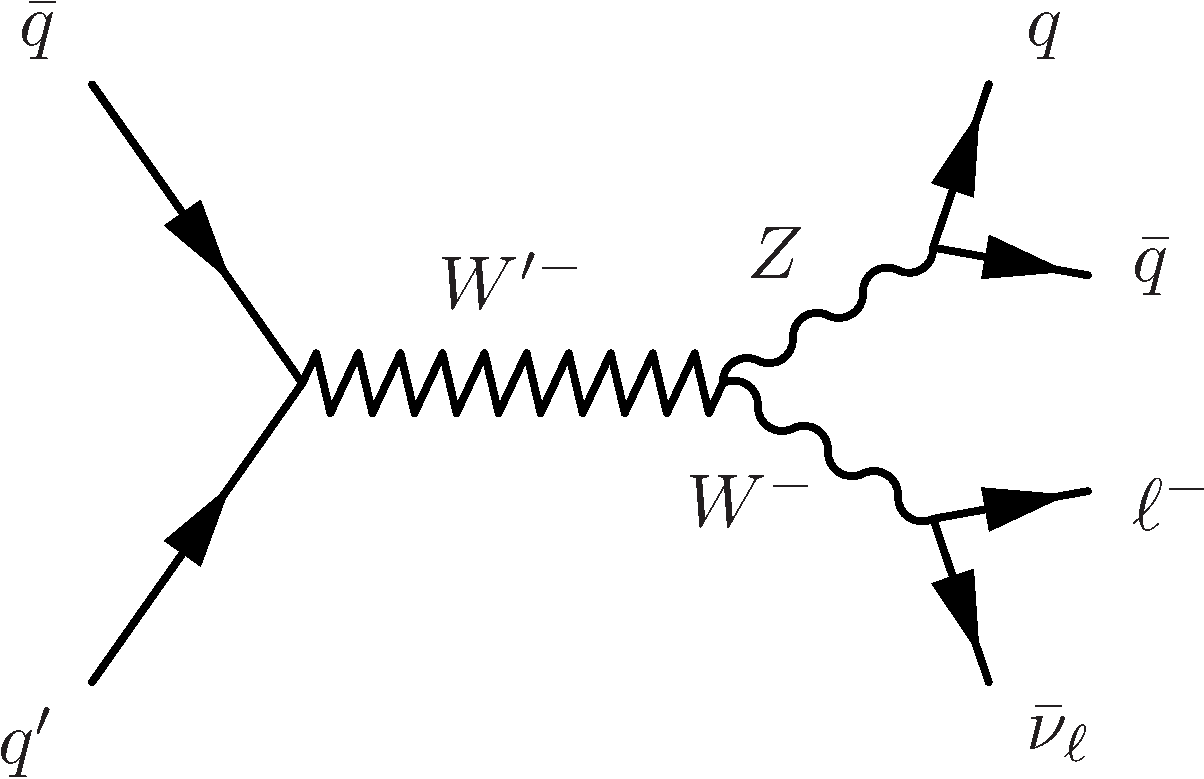
\includegraphics[width=0.3\textwidth]{\chfour/WprimeWZ_LO.pdf}}
\caption{Feynman diagrams for the production of a neutral spin-2 $G$ (a), and a neutral \Zpr (b) and charged \Wpr (c and d) spin-1 resonances.
All resonances decay to a pair of bosons (WW, WZ, or WH) with their subsequent semi-leptonic decay. Charge conjugate modes for \Wpr production and decay are implied.}
\label{fig:FDsignals}
\end{figure}

The search in the $\ell\Pgn\bbbar$ final state is based pp collision data at $\sqrt{s} = 8\TeV$ collected in 2012 and corresponding to an integrated luminosity of 19.7\fbinv.
The second analysis described in this thesis and focused on the $\ell\Pgn\qqbar$ final state is instead based on the pp collision data at $\sqrt{s} = 13\TeV$
collected in 2015 and corresponding to an integrated luminosity of 2.3\fbinv.
Although different algorithms are used for the reconstruction and identification of the hadronically decaying boson, the analysis strategy is similar in the two searches.\\

The key challenge of these analyses is the reconstruction of the highly energetic decay products.
Since the resonances under study have masses of $\approx$~TeV, their decay products, i.e. the bosons,
have on average transverse momenta of several hundred GeV or more.
As a consequence, the particles emerging from the boson decays are very collimated.
In particular, the decay products of the bosons cannot be resolved using the standard algorithms,
but are instead reconstructed as a single jet object. Dedicated techniques, so-called jet ``V tagging'' and ``H tagging'' techniques,
are applied to exploit the substructure of such jet objects, and can help resolve jet signatures of massive bosons.
In particular, the jet is tagged as coming from a V or H boson through the estimation of its invariant mass.
These techniques also help to suppress SM background, which mainly originates from the production of W bosons in association with jets (W+jets).
Further discrimination is achieved in the $\ell\Pgn\bbbar$ analysis channel exploiting the specific characteristics of jets arising from the hadronization of bottom quarks.
As these algorithms aim at tagging V and H bosons of large Lorentz-boost in the final state, a lower limit is placed on the resonance mass hypothesis.
In fact, for values of the resonance mass below 0.6\TeV, the jets arising from the hadronization of the two quarks are not collimated enough to be reconstructed as a single jet,
such that the gain in sensitivity becomes significantly lower. In such cases, analysis techniques exploiting the kinematics of the two resolved jets provide higher sensitivity.
Specifically, the searches in the $\ell\nu\qqbar$ and $\ell\nu\bbbar$ final states are restricted to masses of the mother particle with values above 0.6 and 0.8\TeV, respectively.
A higher value is chosen for the $\ell\nu\bbbar$ search because, being the H boson slightly heavier than the W and Z bosons, it acquires a smaller boost for a given resonance mass.\\

The aim is to reconstruct the full event to be able to search for a localized enhancement in the invariant mass of the WV or WH system on the top of a smoothly falling SM background distribution.
The invariant mass of the WV and WH system is determined by estimating the neutrino transverse momentum with the measured missing transverse energy in the event,
while an estimate of the neutrino longitudinal momentum is derived by imposing the constraint of the W mass on the invariant mass of the $\ell\Pgn$ system.
In the following, the diboson invariant mass will be labelled either \mlvj, or \mWV and \mWH for the $\ell\Pgn\qqbar$ and $\ell\Pgn\bbbar$ final states, respectively.
The SM background mainly comprises W+jets production, although another significant contribution is represented by the production of top quark-antiquark pairs (\ttbar).
Other minor backgrounds are represented by single top quark and SM diboson (WW, WZ or ZZ) production processes.
The Feynman diagrams for W+jets, \ttbar, single top quark and SM diboson production processes are shown, respectively, in Figures~\ref{fig:FDbkgWJets}, \ref{fig:FDbkgttbar}, \ref{fig:FDbkgStop}, and \ref{fig:FDbkgVV}.
The mass spectrum for the dominant W+jets background is estimated from observed events with a reconstructed jet mass not compatible with the V or H hypothesis.\\ 
%This strategy partially relies on the simulation of the background processes.
%Furthermore, simulated events are used for the optimization of the analysis selection aimed at maximizing the discrimination of the signal against the background and hence the analysis sensitivity.\\

\begin{figure}[!htb]
\centering
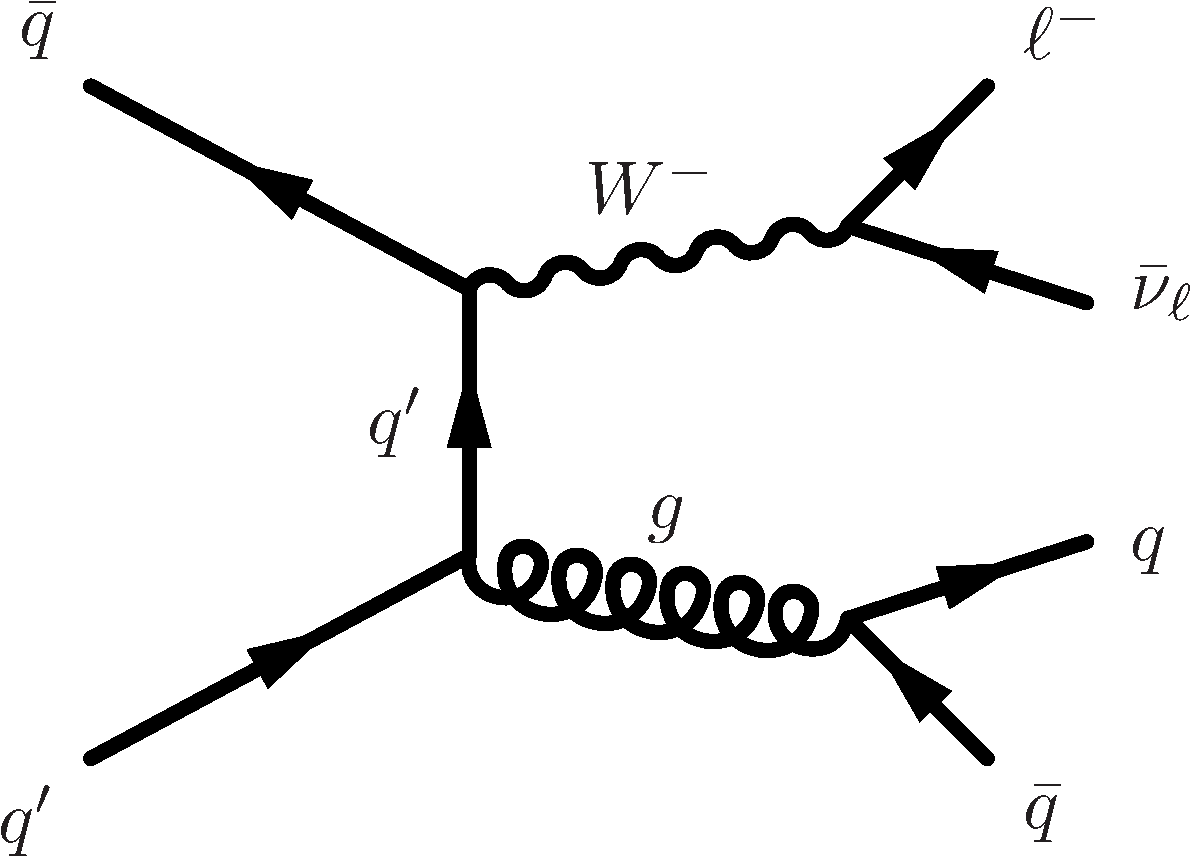
\includegraphics[width=0.3\textwidth]{\chfour/WplusJets_NLO_1.pdf}
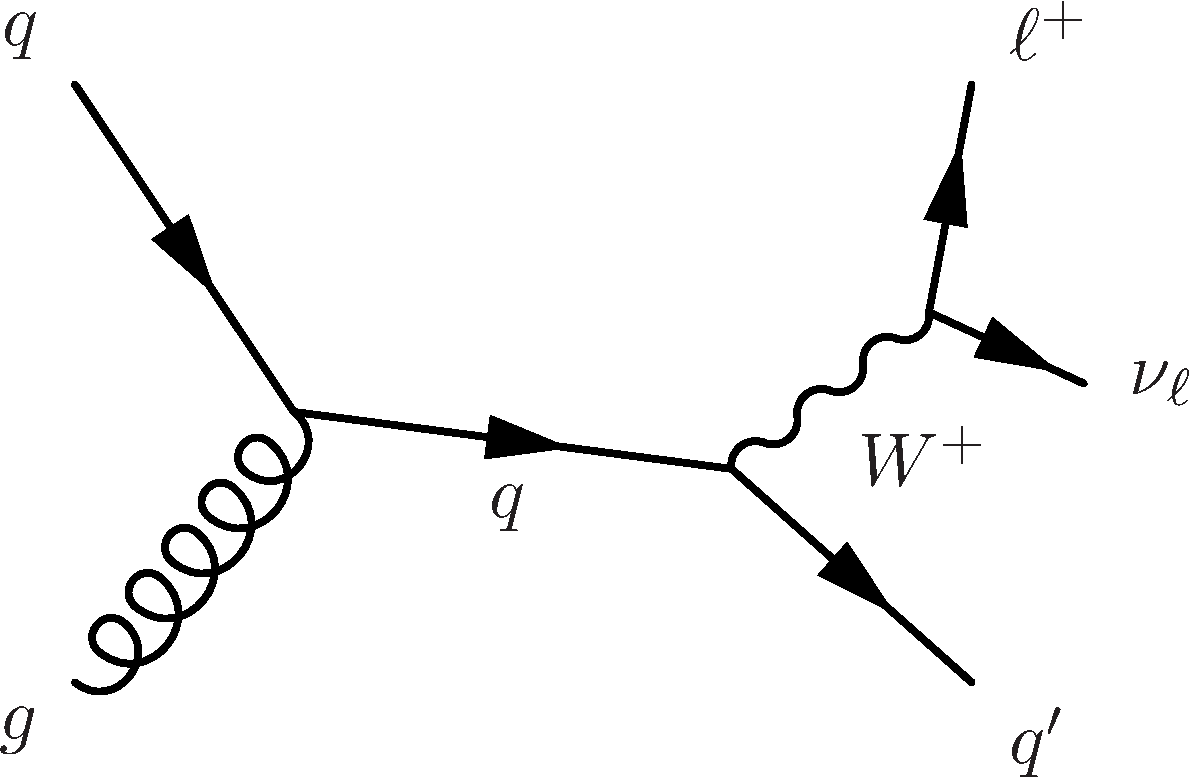
\includegraphics[width=0.3\textwidth]{\chfour/WplusJets_NLO_2.pdf}
\caption{Feynman diagrams for the production of W bosons in association with jets and subsequent decay in the lepton+jet final state. Charge conjugate production and decay modes are implied.}
\label{fig:FDbkgWJets}
\end{figure}

\begin{figure}[!htb]
\centering
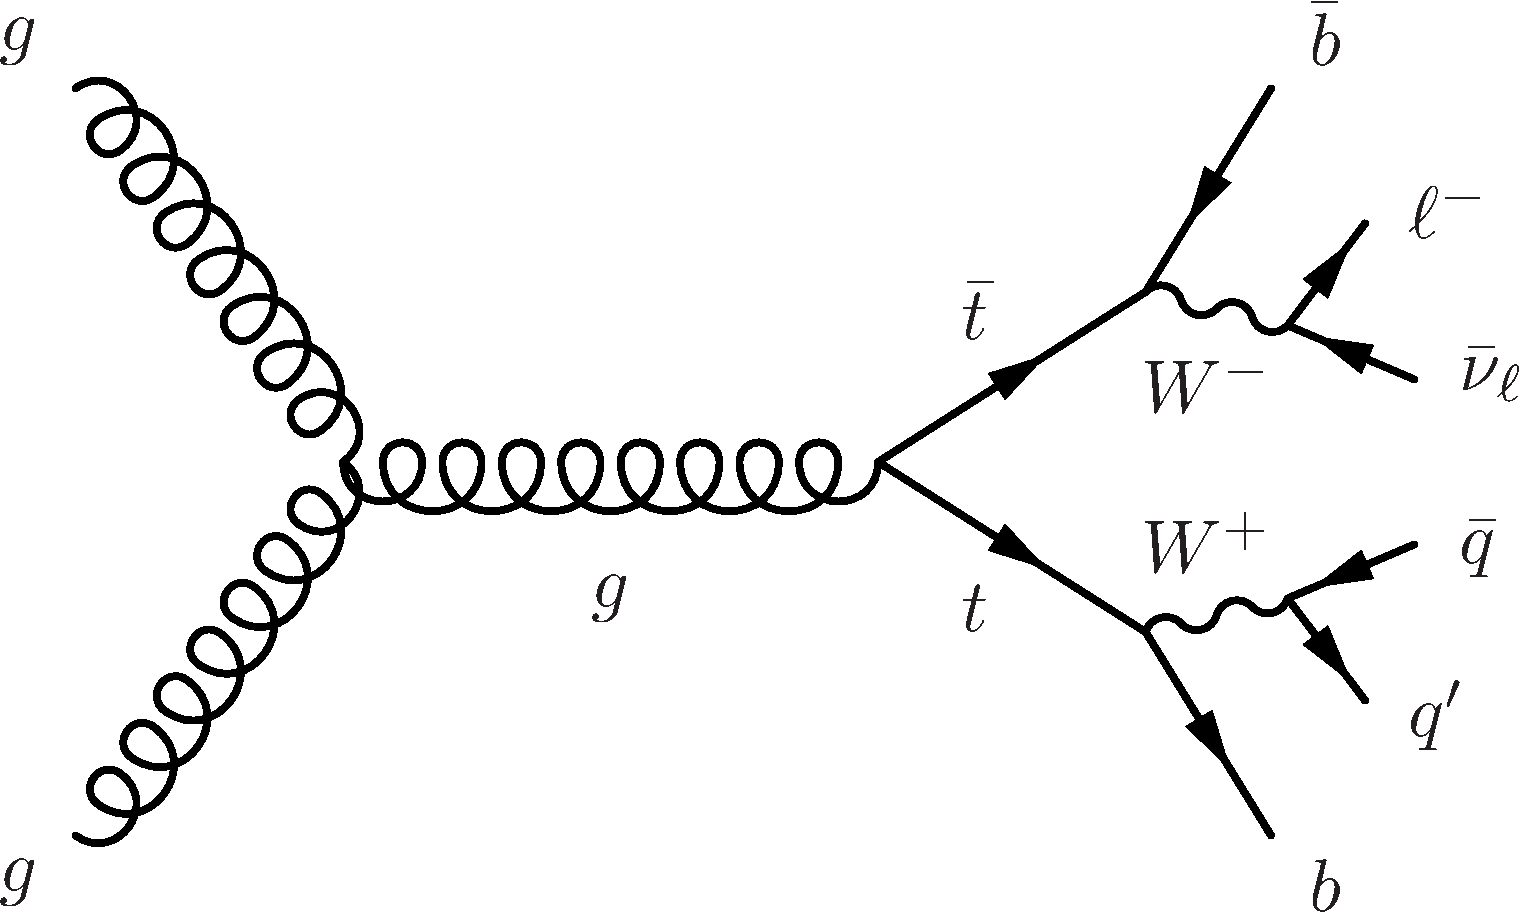
\includegraphics[width=0.3\textwidth]{\chfour/gg_ttbar-1.pdf}
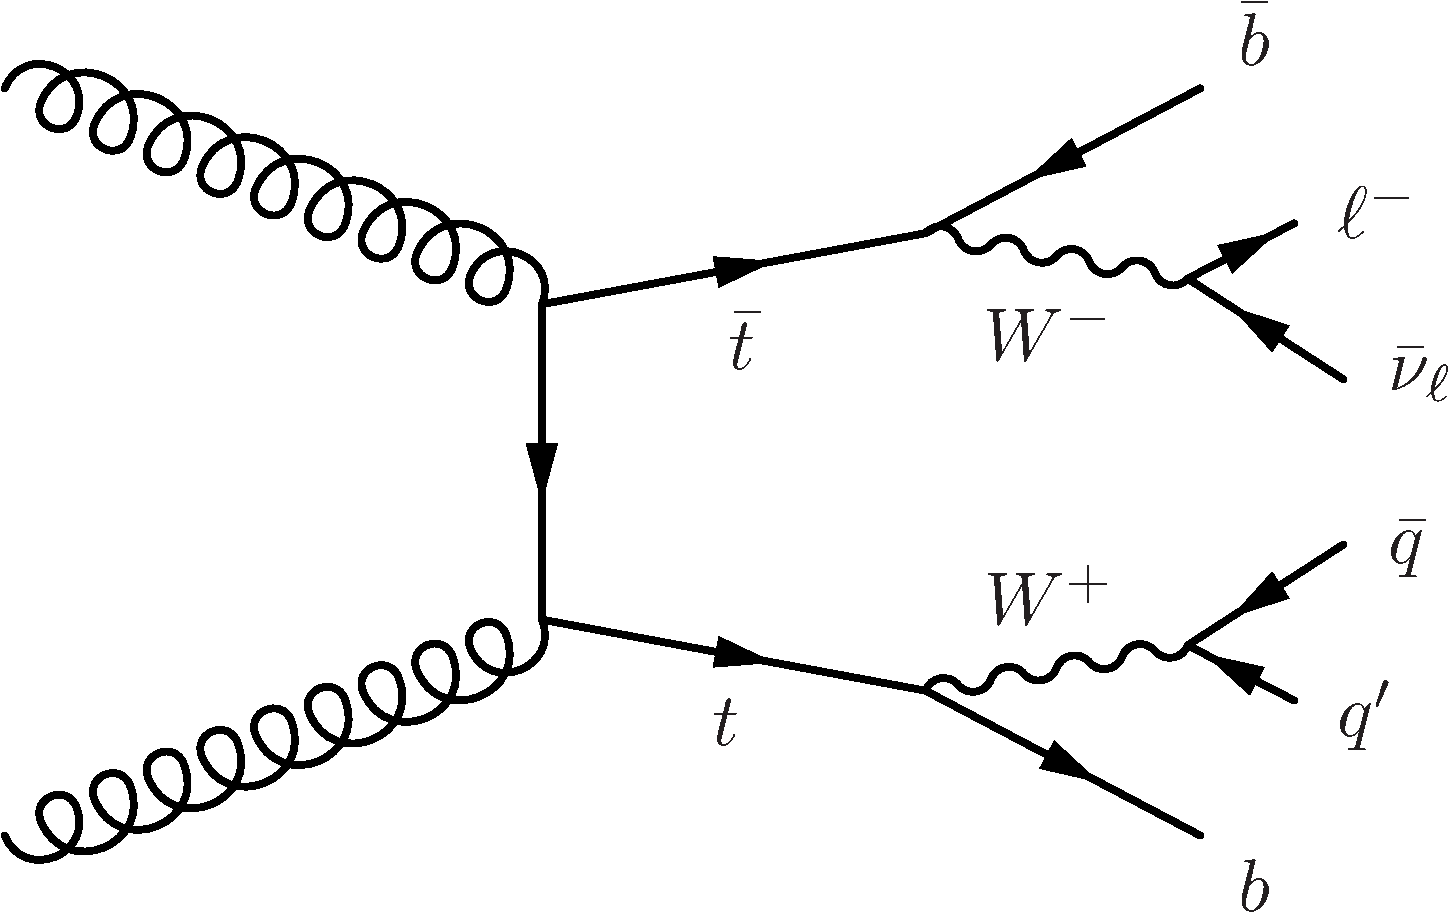
\includegraphics[width=0.3\textwidth]{\chfour/gg_ttbar.pdf}
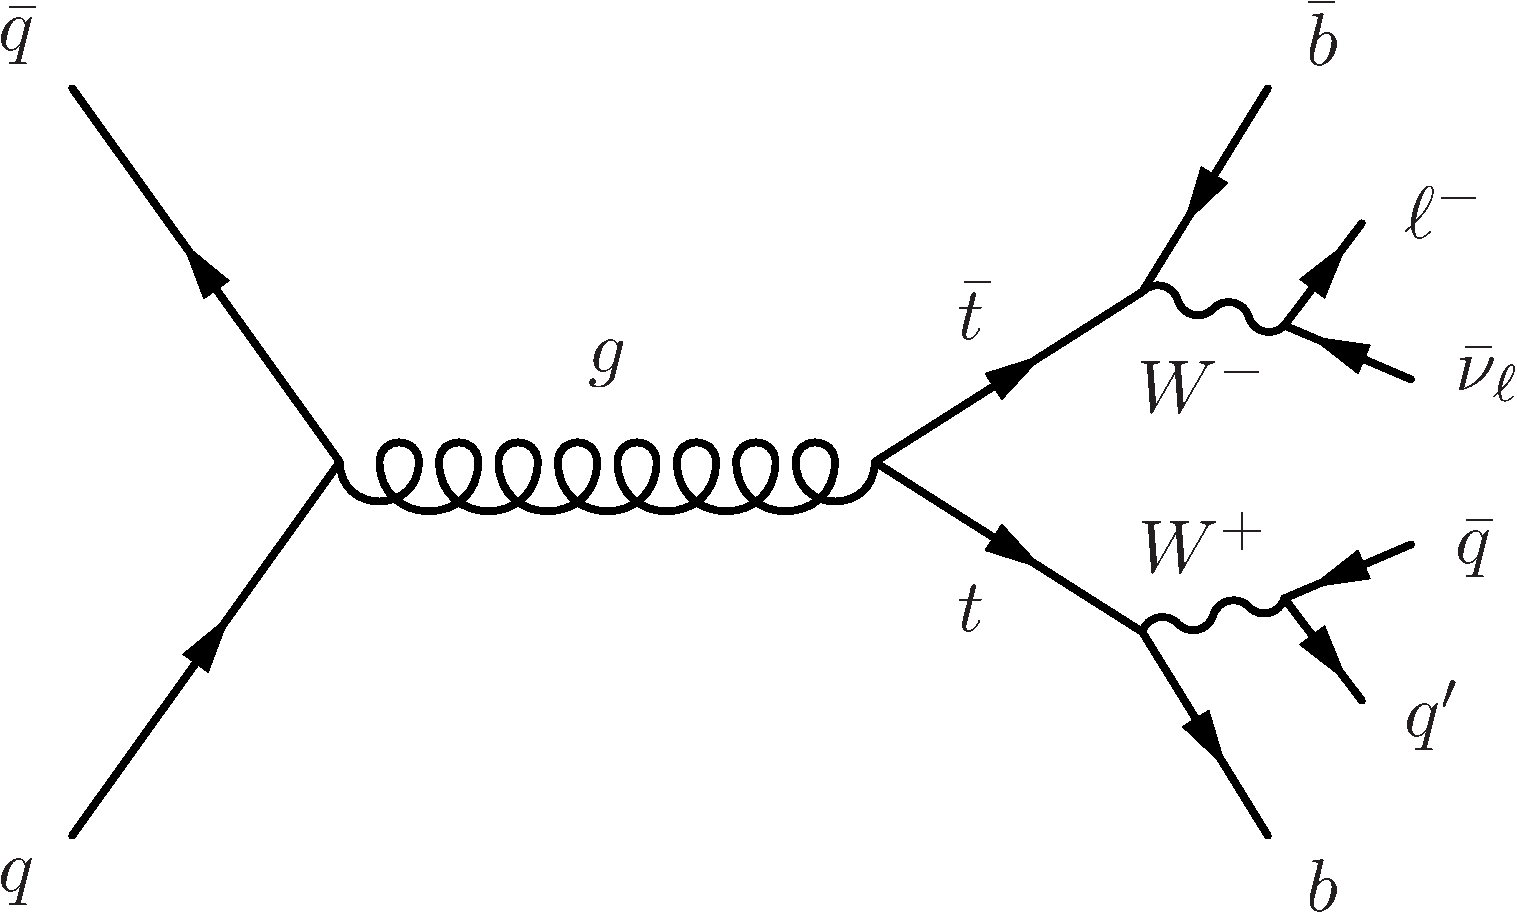
\includegraphics[width=0.3\textwidth]{\chfour/qq_ttbar.pdf}
\caption{Feynman diagrams for the production of top quark-antiquark pairs and subsequent decay in the lepton+jet final state. Charge conjugate modes for the decays of W bosons are implied.}
\label{fig:FDbkgttbar}
\end{figure}

\begin{figure}[!htb]
\centering
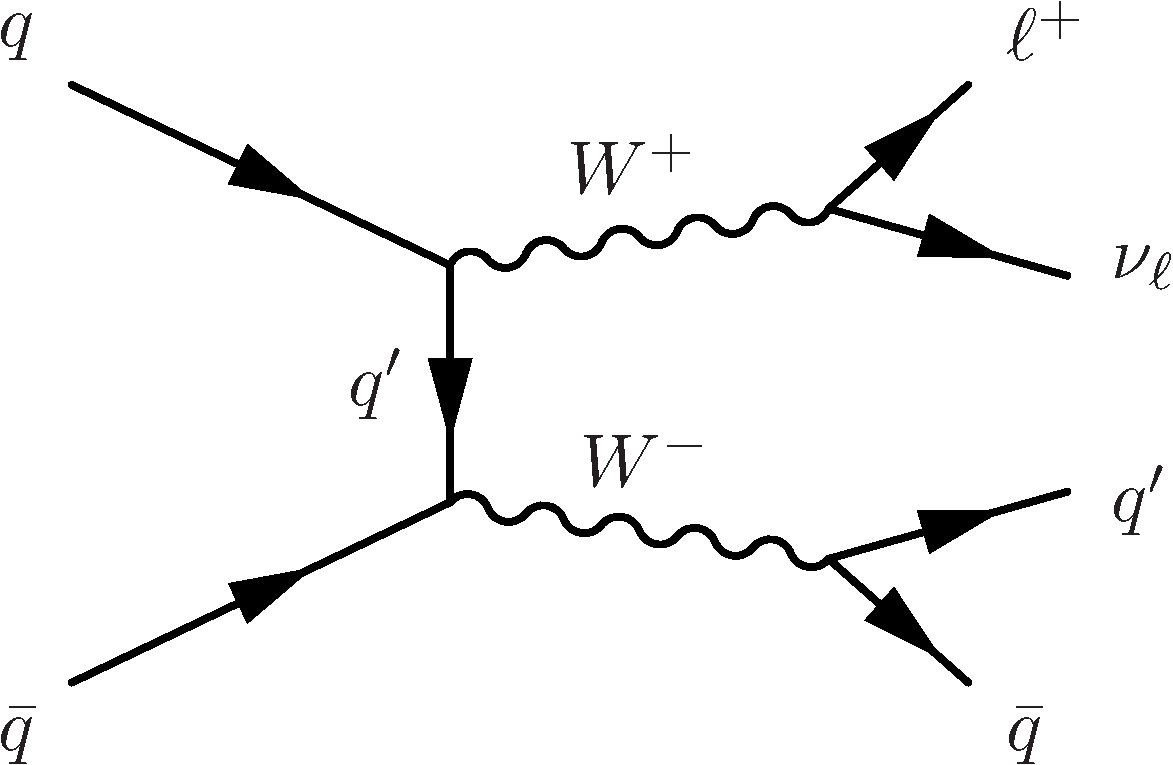
\includegraphics[width=0.3\textwidth]{\chfour/WWproduction.pdf}
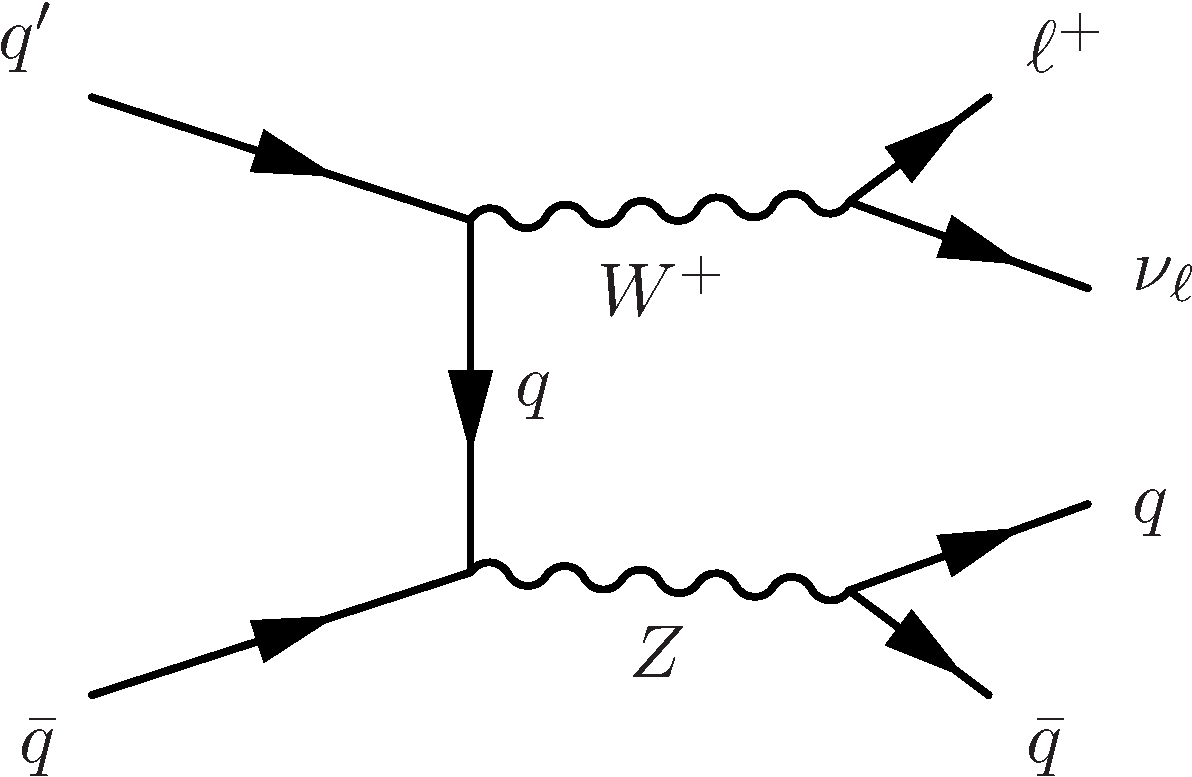
\includegraphics[width=0.3\textwidth]{\chfour/WZproduction.pdf}
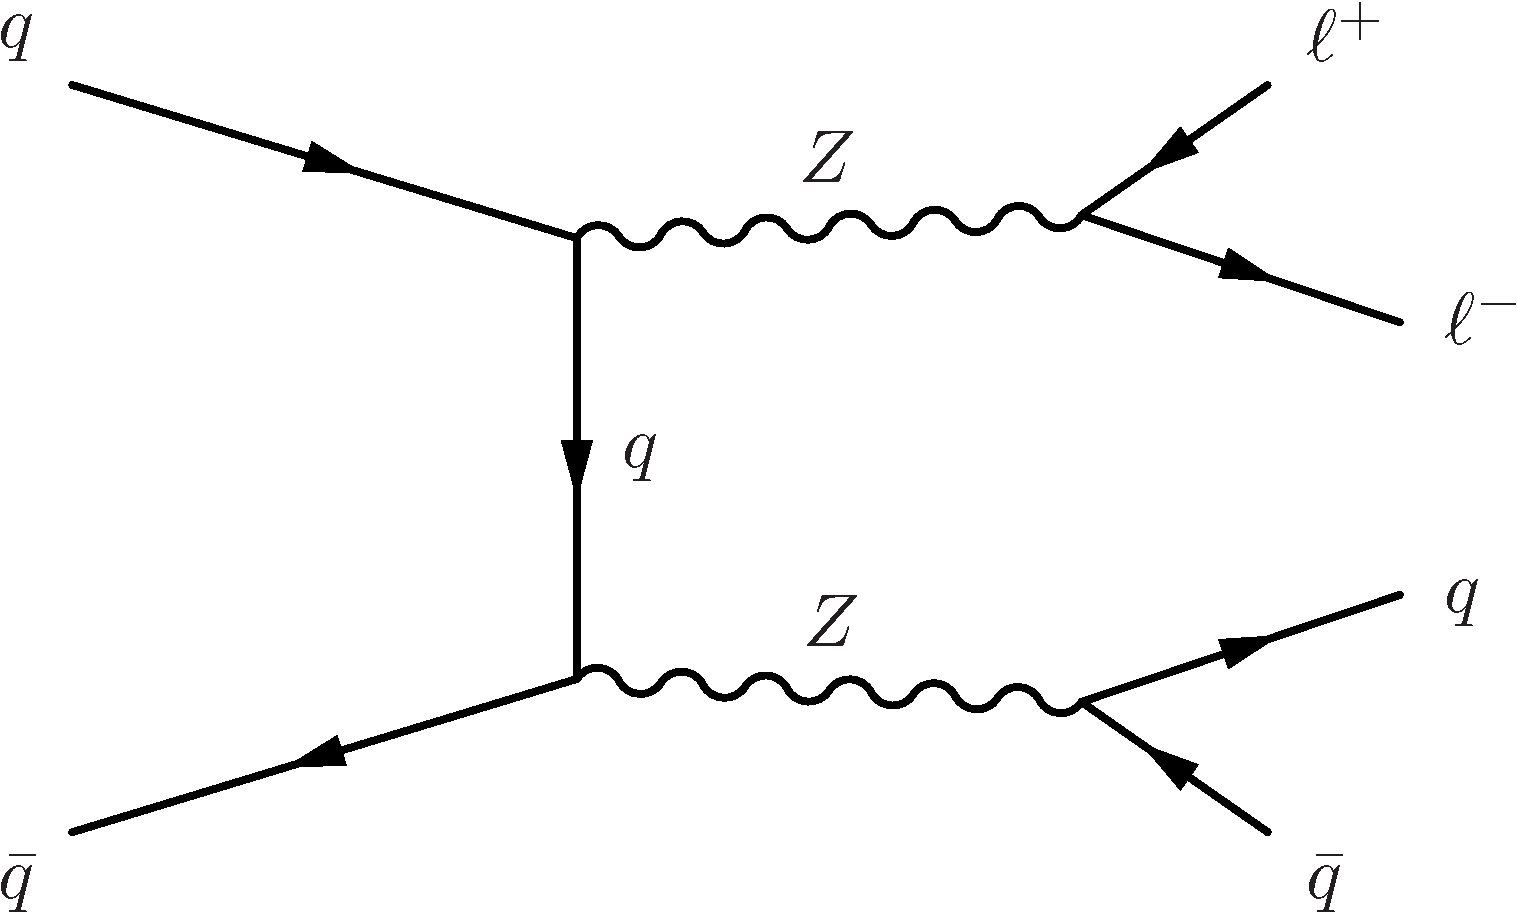
\includegraphics[width=0.3\textwidth]{\chfour/ZZproduction.pdf}\\
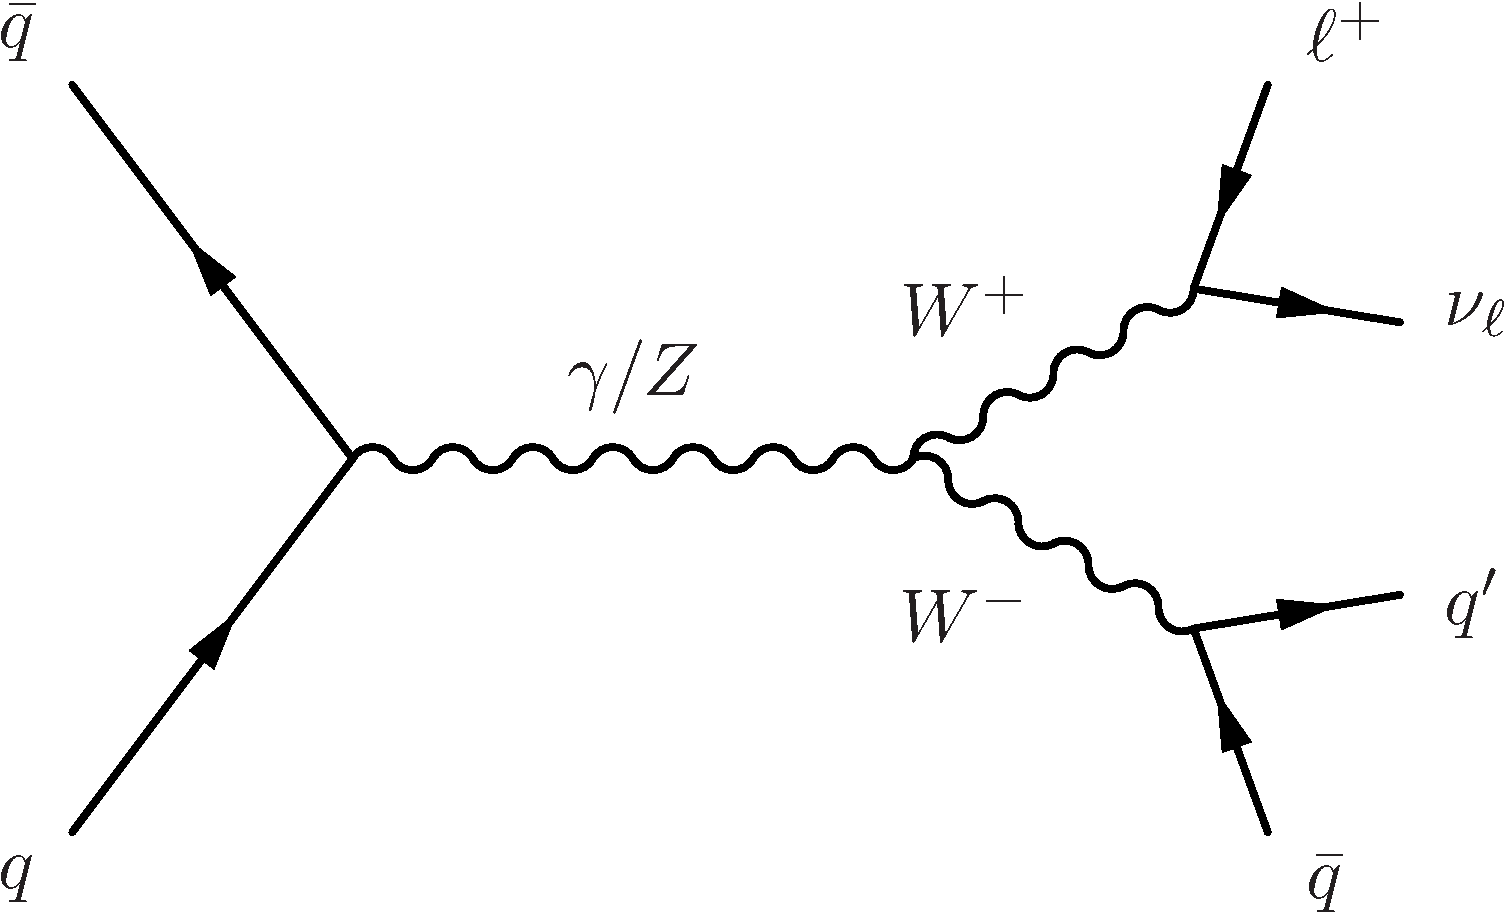
\includegraphics[width=0.3\textwidth]{\chfour/WWproduction-1.pdf}
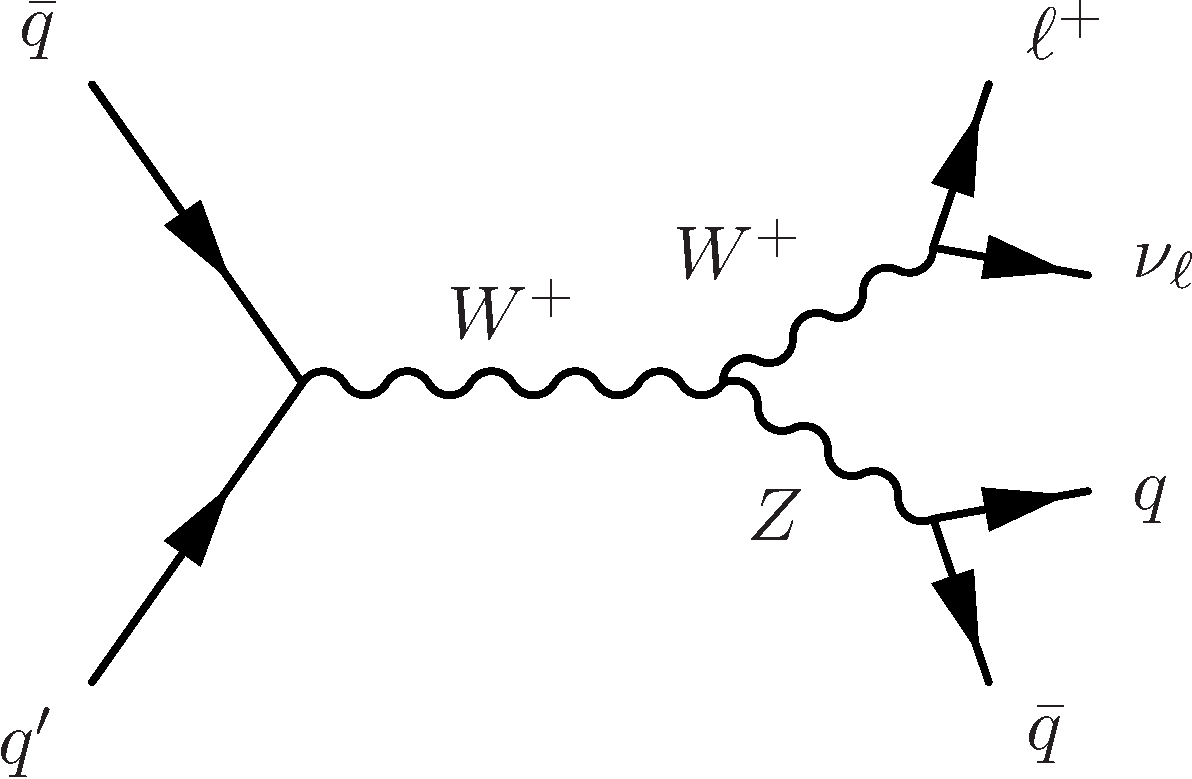
\includegraphics[width=0.3\textwidth]{\chfour/WZproduction-1.pdf}
\caption{Feynman diagrams for the production of SM vector boson pairs and subsequent decay in the lepton+jet final state. Charge conjugate production and decay modes are implied.}
\label{fig:FDbkgVV}
\end{figure}

\begin{figure}[!htb]
\centering
\subfigure[]{\label{fig:FDbkgStop_a}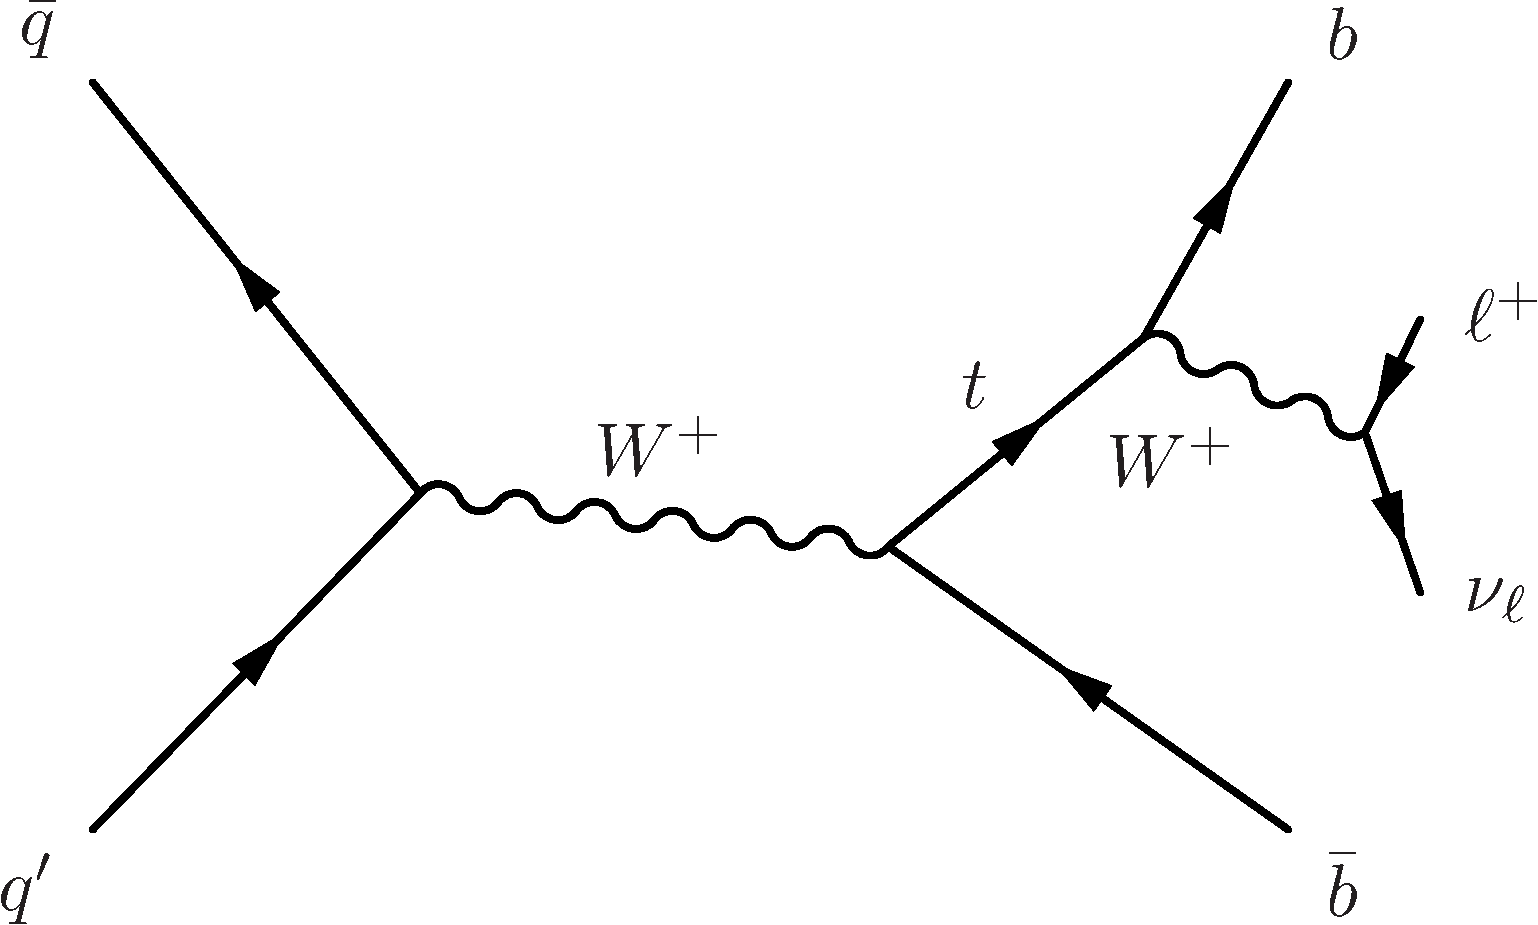
\includegraphics[width=0.3\textwidth]{\chfour/top-schannel.pdf}}
\subfigure[]{\label{fig:FDbkgStop_b}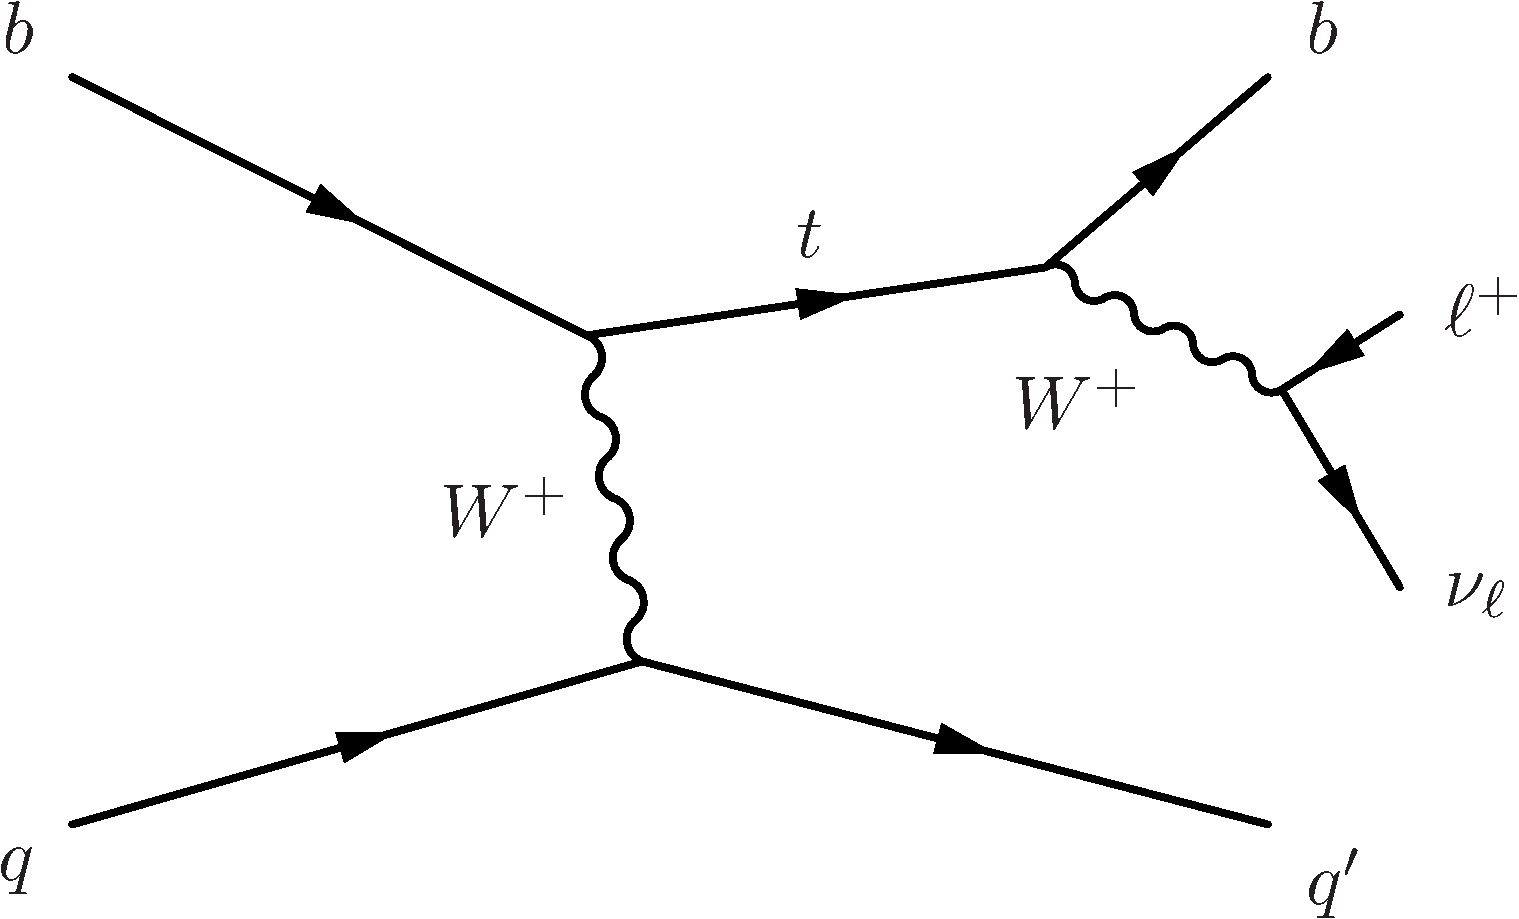
\includegraphics[width=0.3\textwidth]{\chfour/top-tchannel.pdf}}
\subfigure[]{\label{fig:FDbkgStop_c}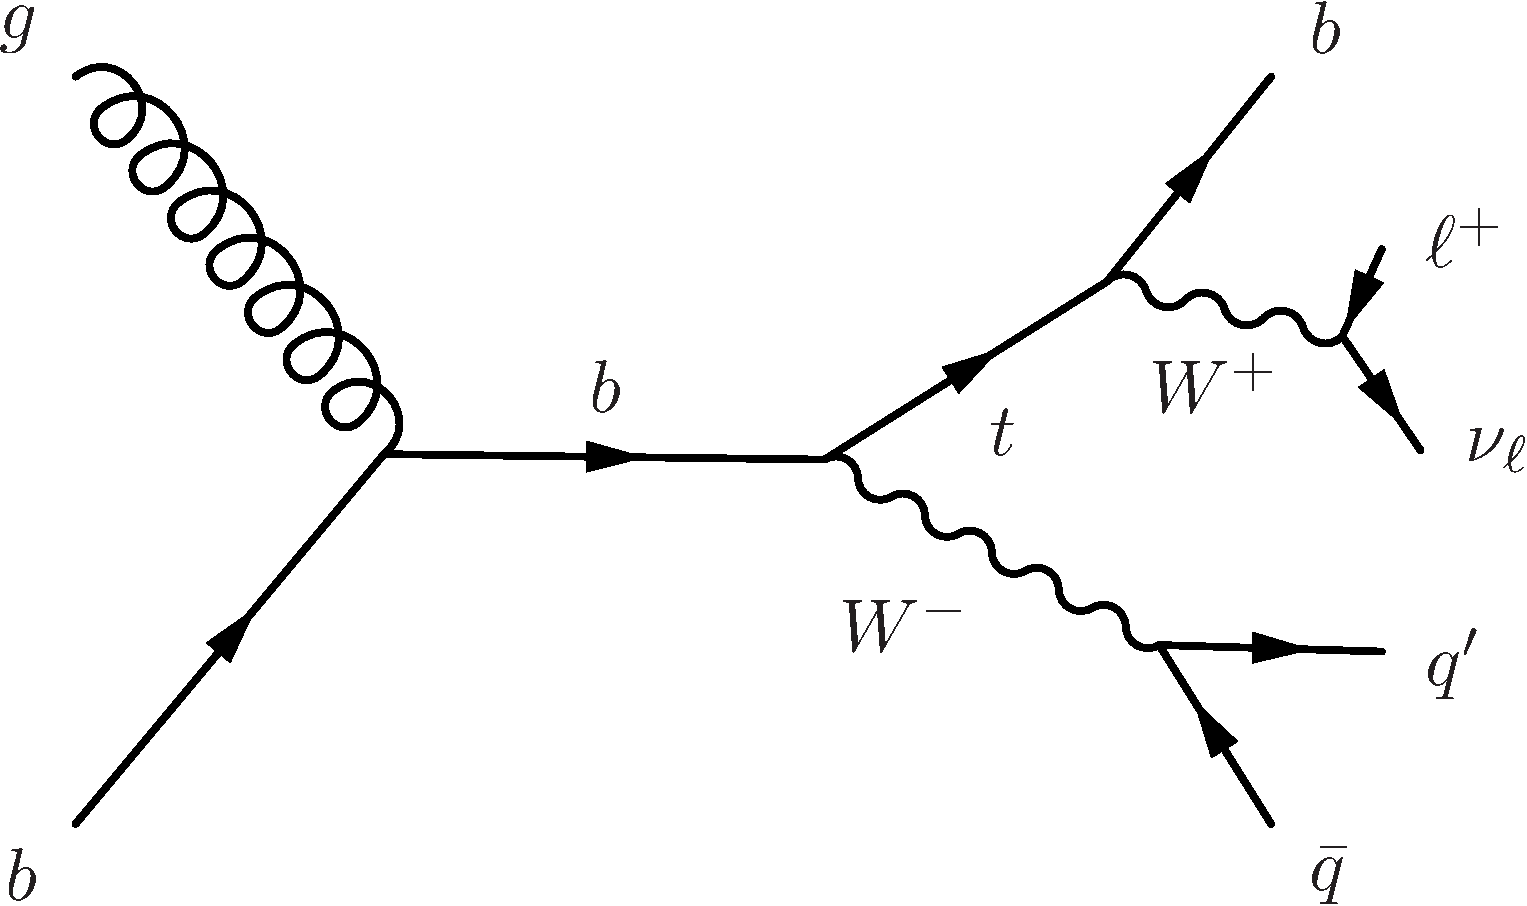
\includegraphics[width=0.3\textwidth]{\chfour/top-tWchannel.pdf}}
\caption{Feynman diagrams for the production of single top quarks and subsequent decay in the lepton+jet final state: (a) s-channel, (b) t-channel, (c) tW-channel.}
\label{fig:FDbkgStop}
\end{figure}

This part of the thesis is organized as follows.
Chapter~\ref{ch:dataAndSim} gives an overview of the methods used to simulate the physics processes happening in pp collisions at the LHC
together with a description of the specific simulated background and signal events used in this analysis, as well as a discussion about the data sets analyzed.
Chapter~\ref{ch:EventReconstruction} provides a detailed description of the algorithms used in CMS for the reconstruction of the event and of the physics objects expected in the lepton+jet final states under investigation.
Particular attention is given to the V and H tagging algorithms representing the key feature of this analysis and therefore, separately discussed in Chapter~\ref{ch:vtagging}.
The analysis strategy, already outlined here, is explained in details in Chapter~\ref{ch:strategy}.
This includes the final event selection and categorization optimized to enhance the analysis sensitivity,
as well as the strategy for the estimation of the expected background, the modelling of the signal and the related systematic uncertainties
which will be used as input to the statistical analysis of the diboson invariant mass distribution observed in data.
The final results are discussed in Chapters~\ref{ch:results8} and~\ref{ch:results13} for the 8 and 13\TeV data analysis, respectively. 
Eventually, these results are combined with limits derived in companion CMS searches for resonances decaying to a pair of bosons in several different final states, with data collected in both LHC Run~1 and Run~2.
%These analyses use the same V and H tagging techniques as presented here to separate the signal from the large multijet or V+jets background.
The statistical combination represent the last piece of this work and it is presented in Chapter~\ref{ch:combination}.